\chapter{Introduction}
\labch{intro}

\section{Context}
In the field of material science, Plastics have been booming since the late 1950s\cite{geyer2017production}.It's a problem for ecosystems, on one hand, by the means of production as 90\% of plastics come from fossil fuels. On other hand,because of its widespread presence in ecosystems gradually degraded into microplastics and nanoplastics. Moreover only 9\% of plastics is recycled and 12\% is incinerated almost all other waste is lost in nature\cite{natureeditorial}.

% \begin{marginfigure}
%     %\centering
%     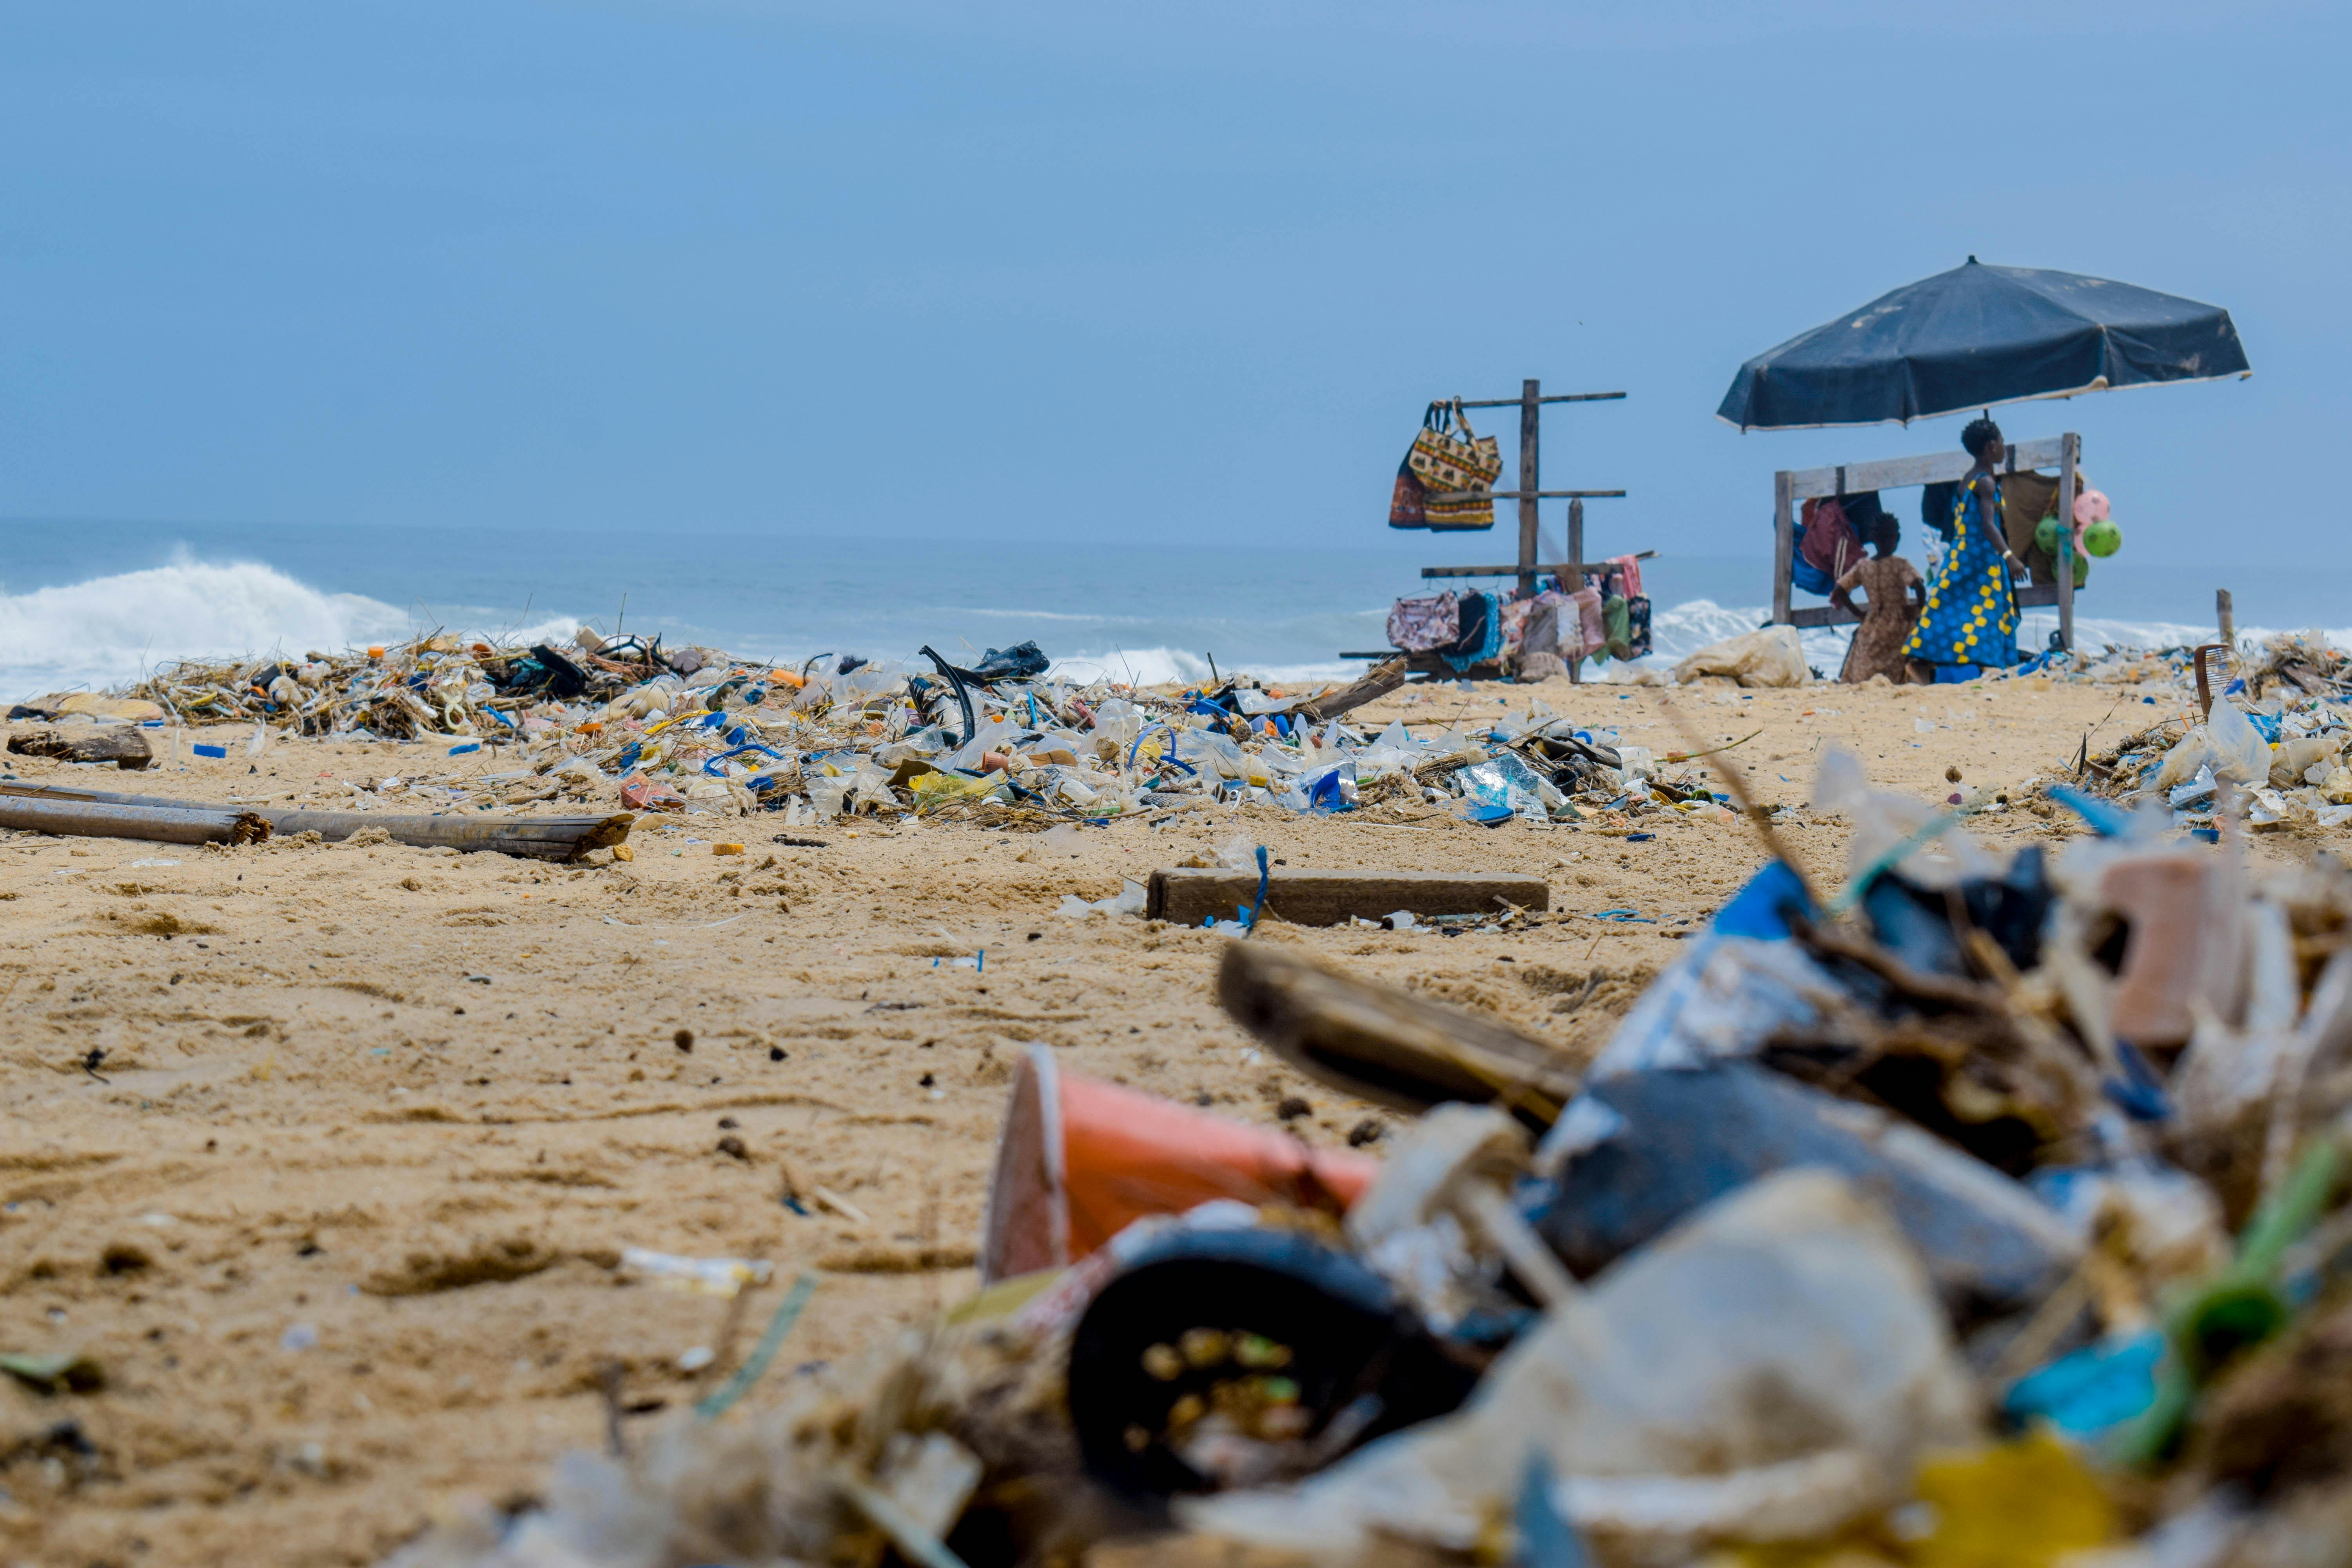
\includegraphics{images/plastic-waste.png}
%     \caption{Plastics pollution on a beach}
%     \label{fig:plastics}
% \end{marginfigure}

\marginnote{
    \centering
    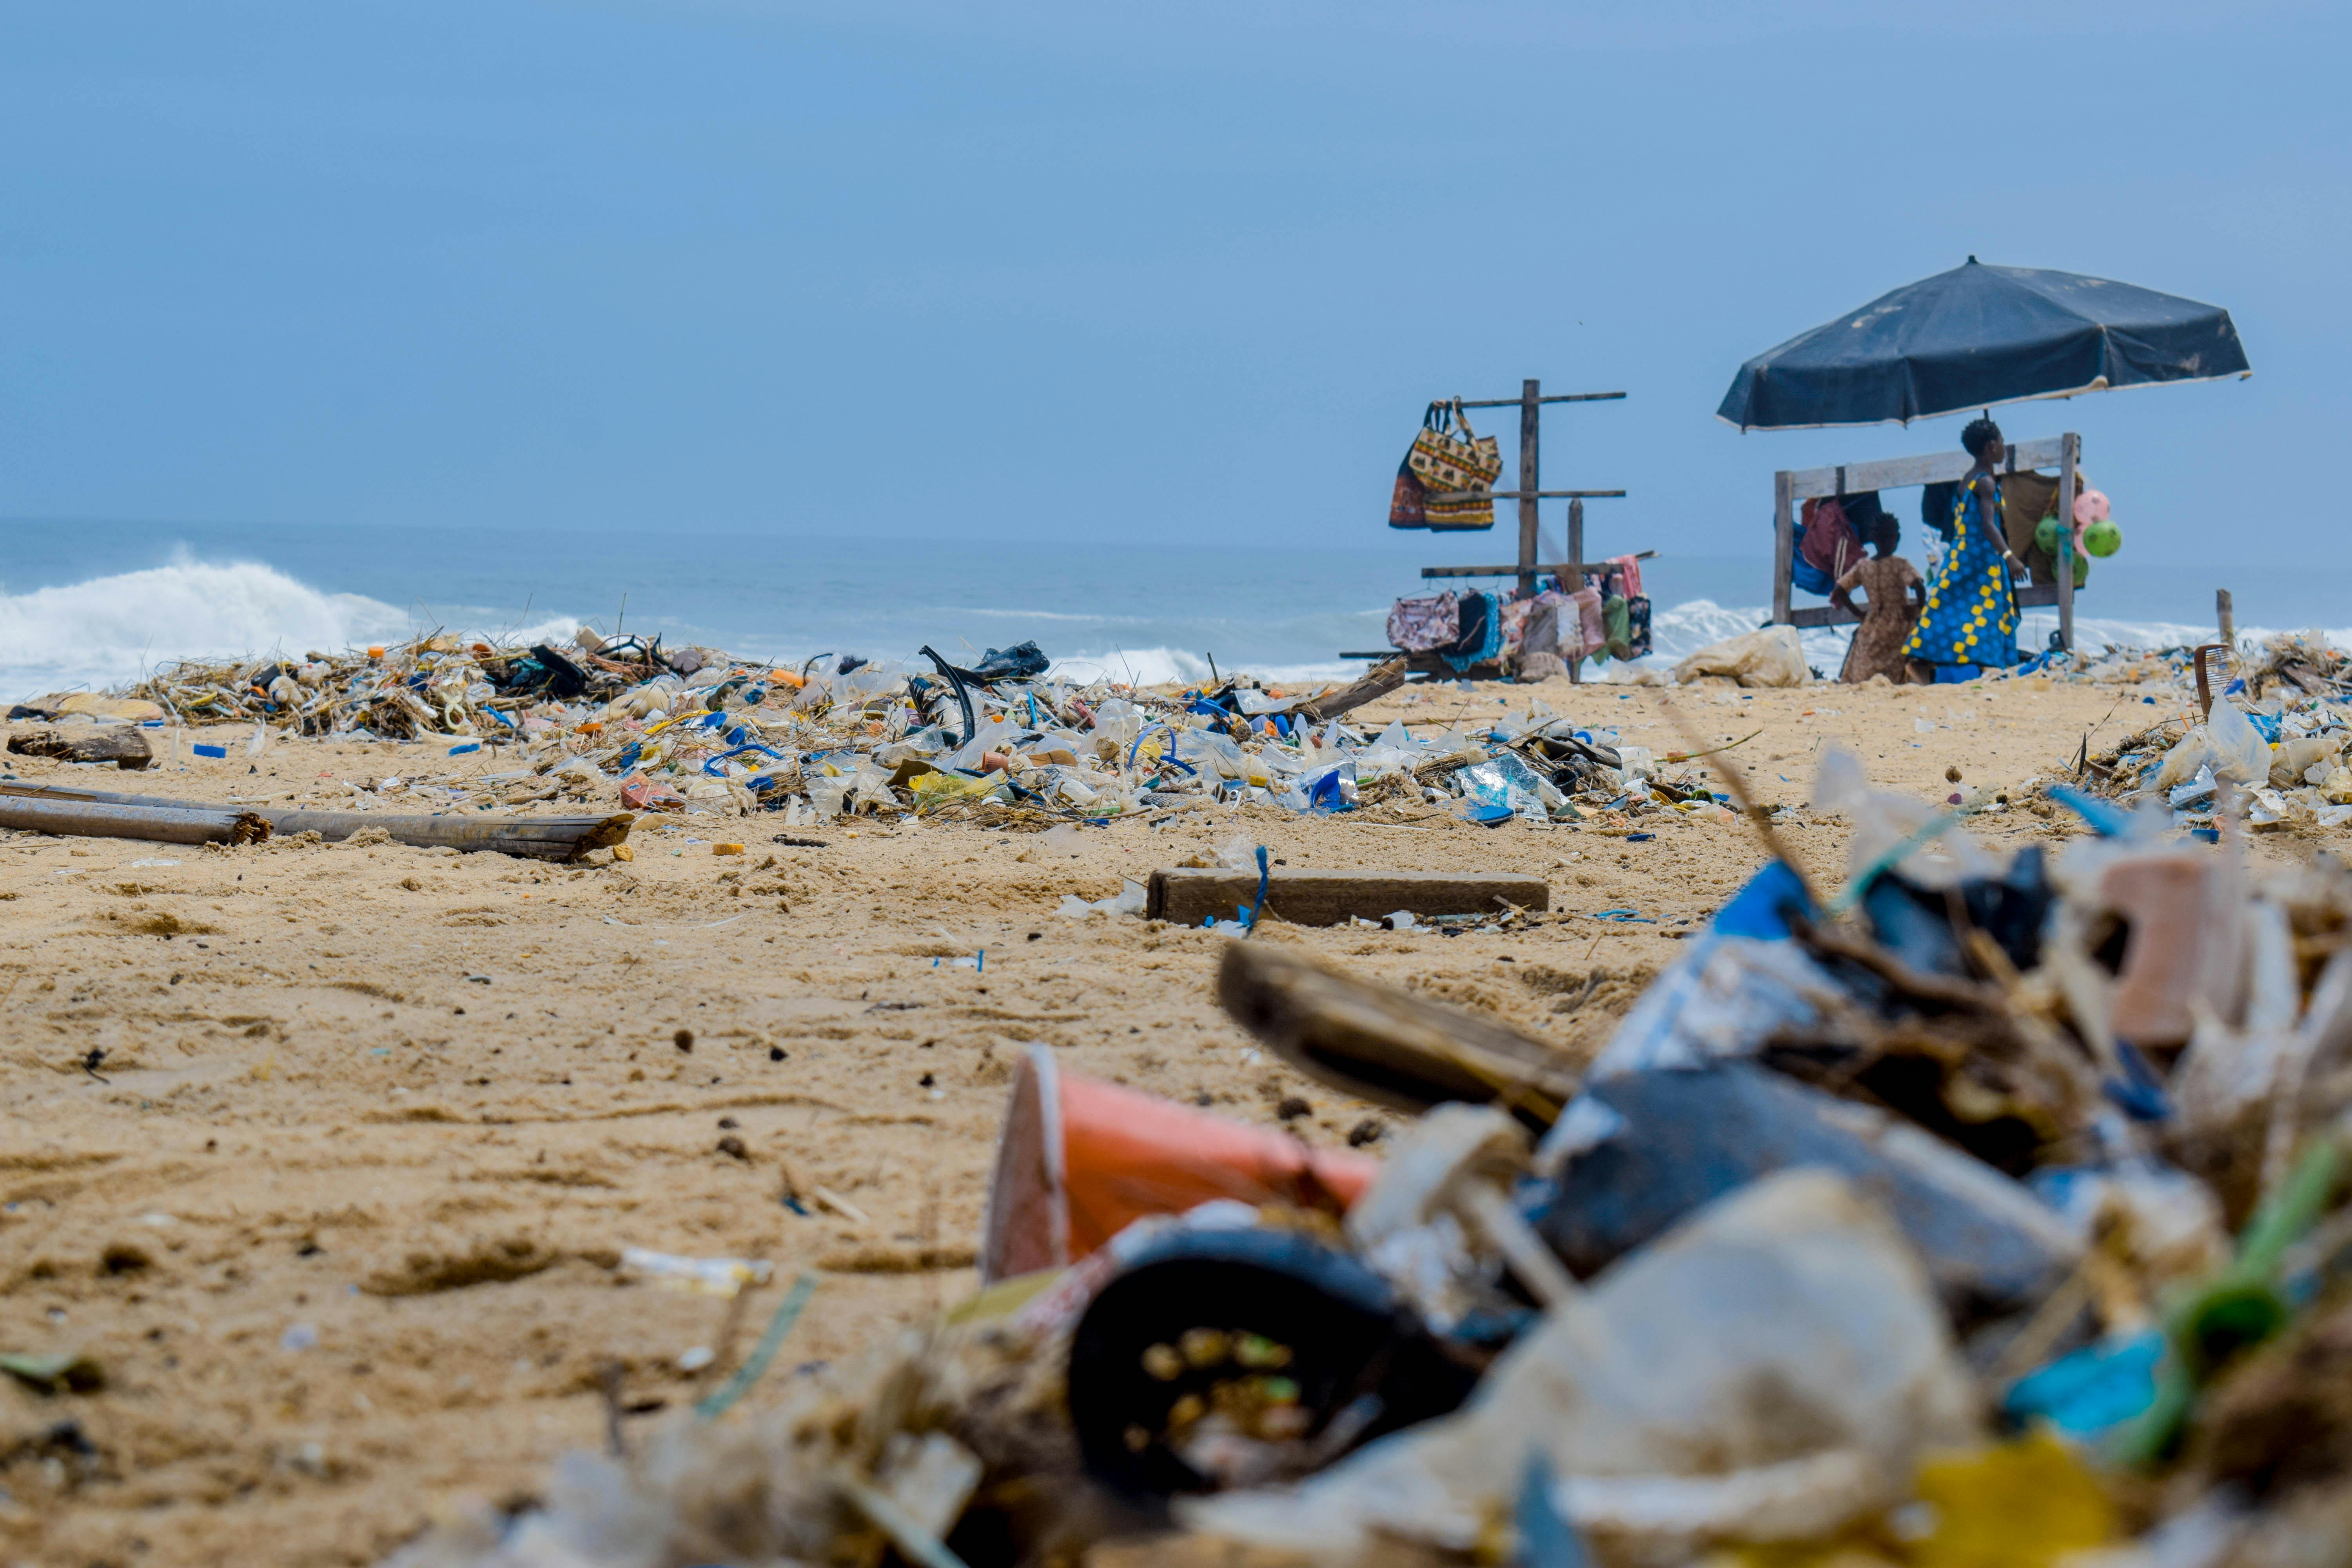
\includegraphics{images/plastic-waste.png}
    \captionof{figure}{Plastics pollution on a beach}
    \label{fig:taele2015maestoso}
}


With plastics, we have a material that our environments can't dissolve and similarly as a a living organism that create it creates an imbalance. Since we have create materials that are "invincible" for the environment,  that environments can't gets rid of, or can't use we've created materials that pollute nature once they're out there.

Moreover we we're moving towards a problem of raw materials in general, independently of plastics. this raises other issues of recycling, delocalization of resources, and the energy needed to extract them from the environment.

That is why, some researcher and designer or other indistrual actor, works on the fabrication of new kind of materials that are biobased.
 
These biosourced materials, which we call biomaterials, have the particularity of being co-created (and sometimes even co-designed) with living organisms. As they are organic materials, this makes them eco-responsible for the environment. 

To makes this kind of biomaterials, it is necessary to understand the living organisms from which it is derived. In order to build machine like controlled environment systems, that reproduces the best growing conditions for our biomaterials.

\section{Approach}
This thesis studies the development and use of biomaterials and the manufacture of a machine tool for biomaterial production.
That is why The areas concerned include biological fermentantion, IOT and sensors, mechanical electronics, and mushroom growth theory. 

Biology is very interesting to make material. In one hand you design new way to create raw materials and be sure that the new materials you create is non toxics for the environment. In other hand, because of the nature of your materials, instead of just creating raw materials you may grow directly concept. 

In both cases, the manufacture of specific controlled environment systems adapted to the biomaterials in question is essential. 
In order to sometimes better understand the growth parameters, optimize biomaterial production, divert or constrain the shape or the way biomaterial grows. 

Furthermore, this thesis also studies the effectiveness and benefits of post-treatment, which may or may not need to be carried out on certain biomaterials 

the general approach is as follows: 

\begin{figure}[h]
    \centering
    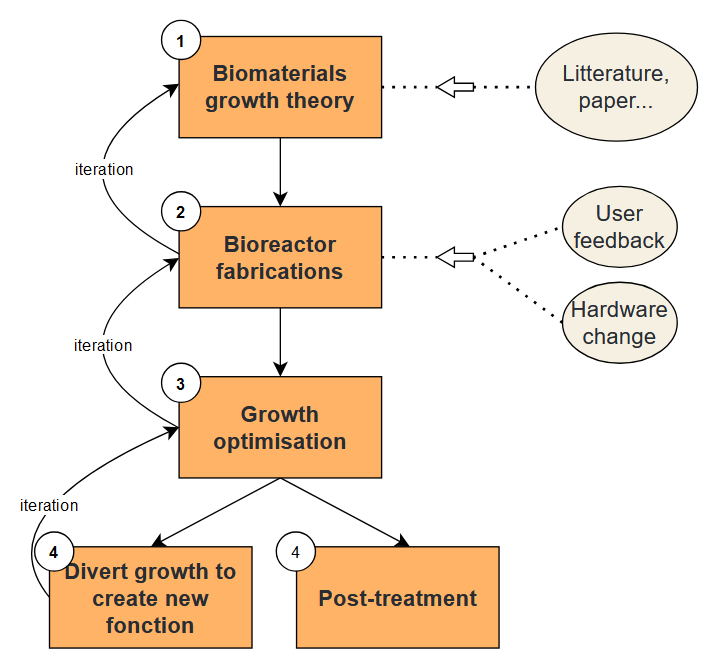
\includegraphics{images/diag_approche.png}
    \caption{General approach overview}
    \label{fig:IS_demo}
\end{figure}


\section{Field of Research}

This research is situated at the intersection of biomaterial science, biological growth processes, and environmental control technologies. Specifically, 
it explores the potential of soft biomaterials such as SCOBY (Symbiotic Culture of Bacteria and Yeast) and mycelium composit, two promising alternatives 
for sustainable material production.

\paragraph[short]{Biomaterial science} 
forms the foundation of this research by investigating the properties, applications, and fabrication processes of materials derived from living organisms. The study of SCOBY and mycelium-based materials is still in its infancy, but early research suggests their high potential for use in sectors such as fashion\cite{amobonye2023fungal}, architecture\cite{ghazvinian2019mycelium}, and packaging\cite{abhijith2018sustainable}, where ecological impacts are a growing concern. And as a substitute for certain materials currently derived from fossil resources\cite{jang2017bacterial}.

matière organique fermentation IOT capteur base de données

dans l'industie 
ecovative 

design 
suzane lee 




\section{Contributions}

my contributions to the field mainly focus on what needs this type of material to be grown and how to optimize it.
And I decide to work on two different types of material. Mycelium and S.C.O.B.Y. 
the goal was to develop a methodology to understand and build machine tools that I use with this kind of growing material. 
The Machine also aim to be ergonomic and useful for the final user. Because all this type of machine might be build simply by just using a box and some kind of actuator.
I decide first to understand the biological process of the material to understand with needs I can control and witch constrained part of the biomaterial I can focus to make 
this material use full to build machine tools in that optimize the process of making them. 